\newpage
\section{RESEARCH METHODOLOGY} 
\subsection{Introduction}
The basic structure for this research work is presented in this section. This section presents the research design, along with conceptual framework, detailing how the research work has been conducted to achieve the research objectives. Thus, this section contains the details of the research design, conceptual framework, sources of data, tools of analysis, along with operational definition of the variables used in this research.  
\vspace{-5mm}
\subsection{Research Design}
To achieve the objectives of this thesis, the research will employ descriptive and explanatory research design.Firstly, analysis of how local levels of Nepal differ in fiscal, economic, and electoral sense will be conducted through descriptive design. Then for the first objective, to gauge the impact of electorate on performance indicators of LISA, a pooled cross sectional regression will be conducted. This regression will use the data collected from the first local level election in 2017 and the performance scores across variety of local governance behavior, as recorded in LISA database. For the second objective, to gauge the impact of performance scores on the fiscal outcomes, panel regression will be carried out. This regression will use data collected from the LISA database and the fiscal data of each local level as provided by the AG annual reports. 
\vspace{-3mm}
\subsection{Conceptual Framework}
In empirical research, a conceptual framework serves as a critical blueprint that outlines the key variables and their interrelationships. It provides a structured approach to understanding how different factors influence the phenomenon under investigation. The following diagram shows how electoral competition, through electoral accountability, influences the governance scores of the local level of Nepal. The conceptual framework, as shown in the figure \ref{Conceptual Framework step 1}, shows the first step of our research design.
\newpage
\begin{figure}[h]
\centering
\hspace{-1cm}
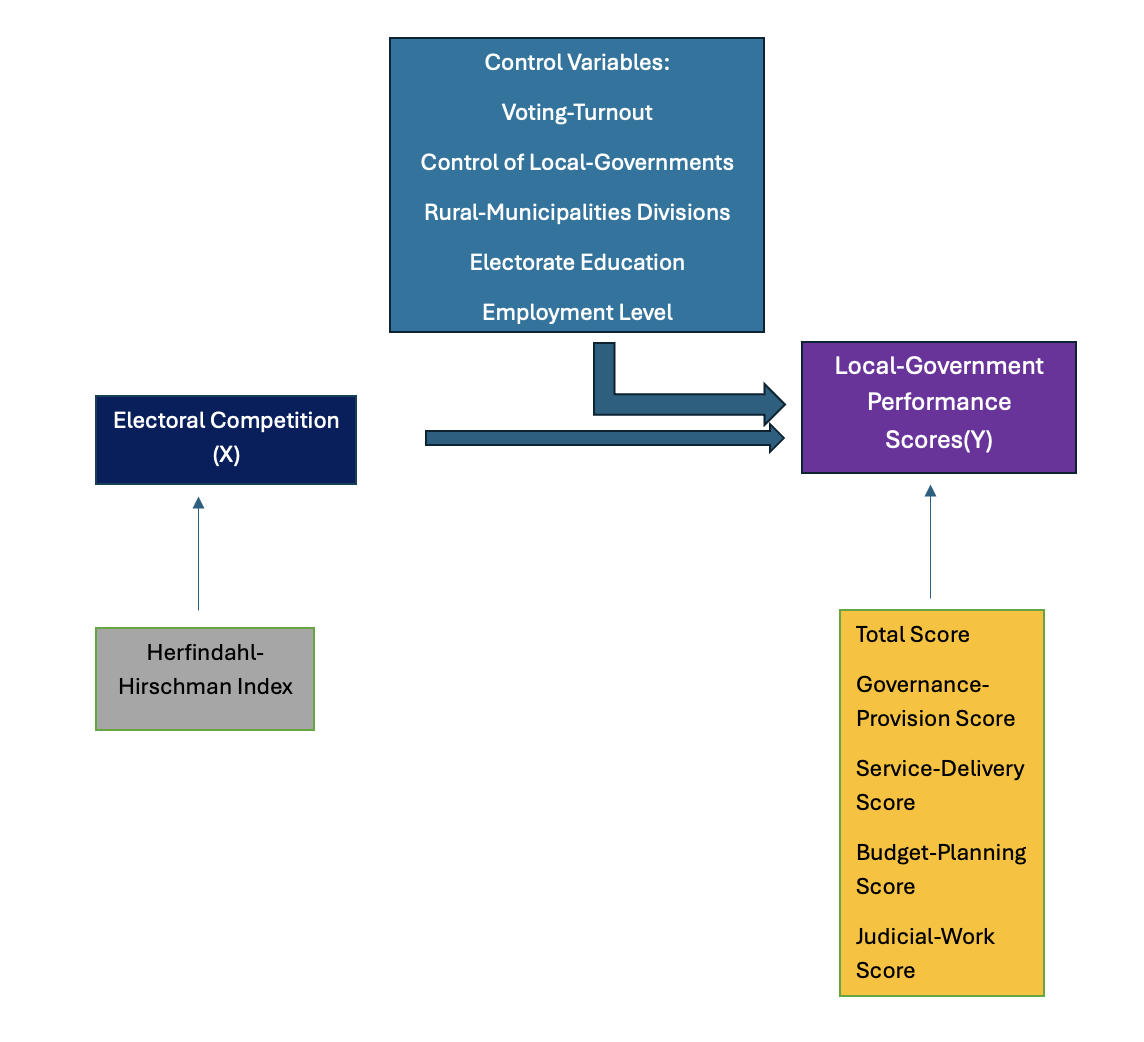
\includegraphics[width = 160mm, scale = 0.35]{figure/Conframe1.png}
\caption{Conceptual Framework of the study-first step}
\label{Conceptual Framework step 1}
\end{figure}
The following figure presents the second step of the conceptual framework, which shows how the governance scores of the local governments translates to the fiscal management. Here, as seen in the figure, the dependent variable of the first step is the independent variables, thus, allowing the study to link up the electoral dynamics with the fiscal management through the governance mechanism.
\begin{figure}[h!]
\centering
\hspace{-1cm}
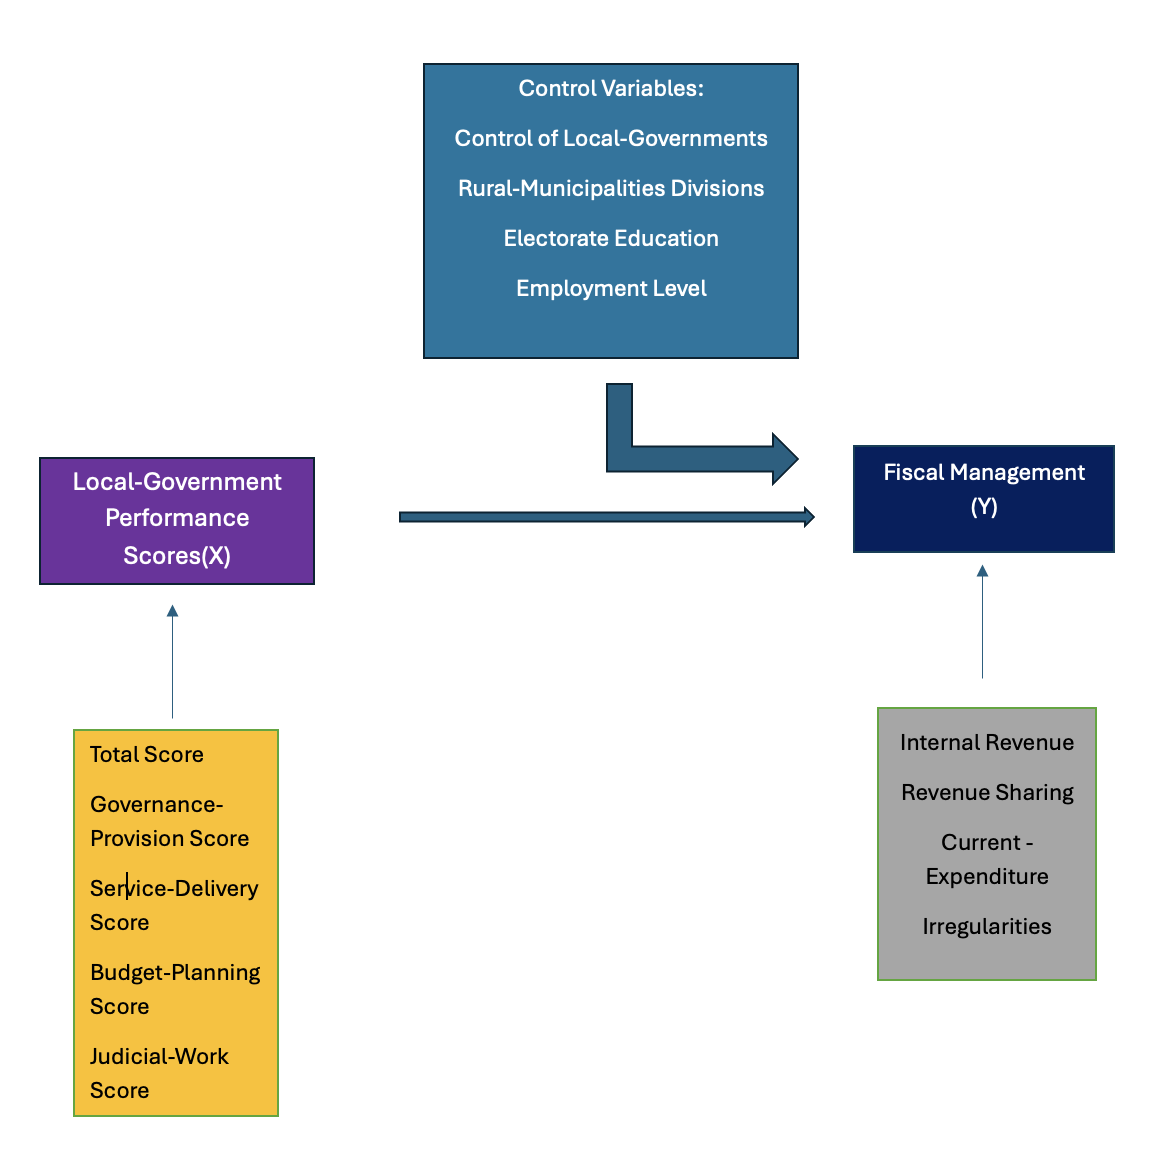
\includegraphics[width = 160mm, scale = 0.35]{figure/Conframe2.png}
\caption{Conceptual Framework of the study-second step}
\label{Conceptual Framework step 2}
\end{figure}

\subsection{Sources of data}
Data have been collected from bevy of sources for this empirical study. The data related to election which are used to construct Herfindahl-Hirschman index and Voting-Turnout variables, were collected from the Election Commission of Nepal website\footnote{election.gov.np} and the official publications of the Election Commission. The data on the status of local levels were collected from the Ministry of Federal Affairs and General Administration\footnote{mofaga.gov.np}. The data on the performance scores of the local governments were taken from the LISA page of the MoFAGA website\footnote{lisa.mofaga.gov.np}  \par
The data on  composition of the local governments were taken from the respective local government websites as well as from the Election Commission, whereas the data on the education status of the local level were taken from the census result of 2021 provided by the CBS. For the fiscal and economic characteristics, including, data on internal revenue each year, income from revenue sharing, current expenditure, and irregularities/Beruju, the data were taken from the annual published report of AG and cross verified through matching it with the respective local levels.
\vspace{-5mm}
\subsection{Operational Definitions of Variables}
The study uses the following variables in the descriptive and explanatory analysis. The Acronym provided here will be used while specifying the model too.\\
\textbf{Herfindahl-Hirschman Index:} HHI is a measure of electoral competition and concentration. It quantifies the level of concentration among mayoral candidates in the 2017 election of Nepal, indicating how evenly or unevenly votes were distributed among them. The score theoretically ranges from 0 to 1, where score closer to 0 indicates the more competitive election while the score closer to 1 indicates more uncompetitive election, where a few candidates dominate the vote share. To make the calculation simple, we only take top four vote receivers, and sum others into another group, where applicable as most constituency did not have more than five candidates.The HHI in our study has been calculated following these steps:\\
\begin{enumerate}[label=\roman*.]  
     \item Obtaining the share of vote of each candidates in the election, thus, dividing the vote received by each candidates by the total vote.
    \item The next step is squaring the vote share of each candidates.
    \item The final step is to sum the squared share of all the candidates of the election. Thus, it could be written as the following formula:
\end{enumerate}
\[HHI =\sum_{i-1}^{n}(s_i)^2\]\\ 
where \(s_i \) is the vote share of the mayoral candidate \( i \), and \( n \) is the total number of candidates.\\
\textbf{Voting-Turnout:} VoteTurnout is, as the name implies, the percentage of total electorate that voted in the election. Thus, the percentage theoretically ranges between 0 to 100, but seldom is 0. \\
\textbf{Control of Local-Governments:} DividedControl, is a dummy variable which indicates if the mayors and deputy mayors are of the same party with the majority of ward members. Thus, it takes a value of 0 if the mayor and deputy mayor are of the same party with the majority of ward members, thus no divided control, and 1 when mayor and deputy mayor are not of the same party, or when they are of the same party but they do not have the majority of ward members of the same party.\\
\textbf{Rural-Municipalities category:} DummyRM, is a dummy variable which indicates if the local jurisdiction is a Rural-Municipality. If the local government is a Rural-Municipality, it is 1 and if it is not, the value is 0.\\
\textbf{Employment percentage:} Employ, is a variable that measures the percentage of people who are employed as per the characterization by CBS. This data is a courtesy of CBS and it is taken as having time-invariant characteristics as the yearly employment data are not available at local levels.\\
\textbf{Electorate Education:} Highedu, is a variable that measures the percentage of people of the local area who have completed intermediate level or more. The data is also a courtesy of CBS, which is based on the 2021 census. Since the education data does not change fast, this study takes the data of 2021 to be applicable to years from 2019 to 2022. \\
\textbf{Total Governance Score:} TotScore, the score as provided by the LISA program for most of the local levels yearly. It is made up of 10 different other scores related to the performance of the government.\\
\textbf{Governance Provision Score:}GovtProv, this score is one of the component of the Total Governance Score as published in the LISA database. This score is normalized to interpret the result better. It shows how the internal local governance structure is organized.\\
\textbf{Service Delivery Score:} ServDeliv, similar to the governance provision score, it is one of the component of the total score and is normalized for better analysis. It shows how the service is rendered by the local governance and is scored as mandated by the LISA operational procedure.\\ 
\textbf{Budget Planning Score:}BudgPlan,  similar to the governance and service delivery score, it is one of the component of the total score and is normalized for analysis. It shows how the annual budget and project planning is carried out by the local governments. \\
\textbf{Judicial Work Score:} PhyInfra,  one of the component of total score, it is normalized for analysis.It shows how the physical infrastructure promotion work of the local governments is carried out during the year. \\
\textbf{Internal-Revenue:} Intrevtot, is a variable that measures the internal income generated by the local level divided by the total revenue of that local level. Thus, this variable gives us what percentage of total revenue of that local level was generated internally by the concerned local level. The study expects that independent variables, governance performance scores, to have a positive association with this variable as when performance value increases, the local level is more willing and able to increase its internal source of income and thus, corresponding rise in the share of internal revenue to total revenue.\\
\textbf{Revenue-Sharing:} Revshrtot, is a variable that calculates the income earned by the local levels as a fraction of their total revenue, from sharing the revenue with the provincial and central government. The study expects positive association with governance performance scores for the same reason as mentioned in Internal-Revenue variable section.\\
\textbf{Current Expenditure:} Curexptot variable is the fraction of the current expenditure of the local level to its total expenditure. The study expects positive association with governance performance scores as increase in HHI means decrease in electoral competition, which could weaken accountability and motivate the elected officials to spend more on current expenditures.\\
\textbf{Irregularities-Beruju:} Berujutot variable measures the `Beruju' of each local level as a percentage of the total expenditure of that local level. Raw comparison of it would not be wise as there are local levels with different stratum of expenditures, thus, per capita technique is applied. 
\vspace{-3mm}
\subsection{Tools of analysis}
\subsubsection{Descriptive Analysis}
This study performs the descriptive analysis of the variable used in the model using statistical tools such as mean, median, and standard deviation to give context to the variables. Thus, in the next section, this study would provide the descriptive statistics of variables like HerfindahI-Hirschman Index, Vote-Turnout, Education level, Internal income of local governments among other variables.
\subsubsection{Explanatory Analysis}
The examination of relationship between electoral competition, as given by HHI, with the variables of fiscal and economic discipline will be carried out. For the first relationship between electoral dynamics and governance performance scores,  the independent variable and control variables are all time-invariant, while the dependent variables of governance performance scores are all time variant, \citeA{Wooldridge2009} and \citeA{Wooldridge2010} states that neither fixed effect regression model nor random effect model could be used as key regressors are time-invariant. While panel structure would have allowed for the analysis of effects across multiple years, this study intends to capture broad, long-term effect and using pooled regression is valid for it. \par
For the second relationship, unbalanced panel regression would be used for analysis as the data are suited for it. Tests would be carried out to see whether fixed or random effect model would better present the relationship between the dependent variables and the independent variables, along with other tests to account for proper model specifications. 
\vspace{-4mm}
\subsubsection{Model Specification}
For the first relationship, this study will be using  pooled cross sectional regression to investigate the relationship between the independent and dependent variables. Since the cross sectional regression merges the panel observations, without taking account of time variation, and would not account for autocorrelations in the residuals, this study runs a pooled regression with the following equation:
\begin{align}
Y_{it} & = \alpha + \beta_1 \text{HHI}_i + \beta_2 \text{VoterTurnout}_i + \beta_3 \text{HighEdu}_i \nonumber \\ &\quad + \beta_4 \text{DumRM}_i + \beta_5 \text{DivControl}_i + \beta_6\text{Employ} + \beta_\gamma D_t + \epsilon_{it} 
\end{align}
Where:\\
- \(Y_{it}\) - Dependent variables(Governance performance scores, including TotScore, GovtProv, ServDeliv, BudgPlan, and PhyInfra,  of local level  i at time  t.)\\
- \(HHI\) (Herfindahl-Hirschman Index) measures political concentration at mayoral level.\\
- \(VoterTurnout\) represents the voting percentage.\\
- \(Divcontrol\) is a dummy variable indicating whether the control of the jurisdiction is divided or not.\\
- \(highedu\) refers to the percentage of highly educated(intermediate or more) individuals.\\
- \(DumRM\) is a dummy variable indicating rural or municipal areas.\\
-\(Employ\) is an employment variable, that is provided by the census of 2078.\\
-\(D_t\) - Dummy variables for the years 2077, 2078, and 2079 (to control for time effects).\\
-\(\beta_\gamma \) -Coefficients for the time dummies.\\
- \(\alpha\) is the intercept.\\
- \(\epsilon\) is the error term.\\
Each coefficient \(\beta_1, \beta_2, \beta_3, \beta_4, \beta_5, \beta_6\) will represent the estimated effect of the corresponding independent variable on the variables of governance performance score.\par
For the second relationship, unbalanced panel regression would be used with the following specification:
\begin{align}
Y_{it} &= \alpha + \beta_1 \text{Governance\_Score}_{it} + \beta_2 \text{Highedu}_i + \beta_3 \text{DivControl}_i \nonumber \\ &\quad + \beta_4 \text{DumRM}_i + \beta_5 \text{Employ}_i + u_i + \epsilon_{it}
\end{align}
Where:\\
- \(Y_{it}\) - Dependent variables showing the fiscal conditions of the local level \emph{i} at time \emph{t}, including Intrevtot, Revshrtot, Curexptot, and Berujutot.\\
-\(Governance\_Score_{it}\) - The chief independent variable is the total governance score of local government \emph{i} at time \emph{t}, as provided by the LISA database.\\
-Other control variables are as explained in equation (1).\\
-\(u_{i}\) represents the unit-specific error term or unobserved heterogeneity. It captures the effects that are specific to each local level but do not vary over time. These could be characteristics that are unique to each local level but are not directly observed or included in the model. It captures unit-specific characteristics that are constant over time(fixed or random effect depending on the model that would be used).\\
-\(\epsilon_{it}\) represents the idiosyncratic error term that captures the time-varying shocks or random errors for each local level at time t. Thus, it contains random shocks or error that are not explained by the independent variables and change over time. \\


